\begin{frame}
    \frametitle{The Problem}

    Given a physical system for which we have some experimental data, can we utilize machine learning to understand the
    physics of the system?
    \bigskip

    \begin{figure}
        \centering
        \begin{subfigure}[b]{0.45\textwidth}
            \centering
            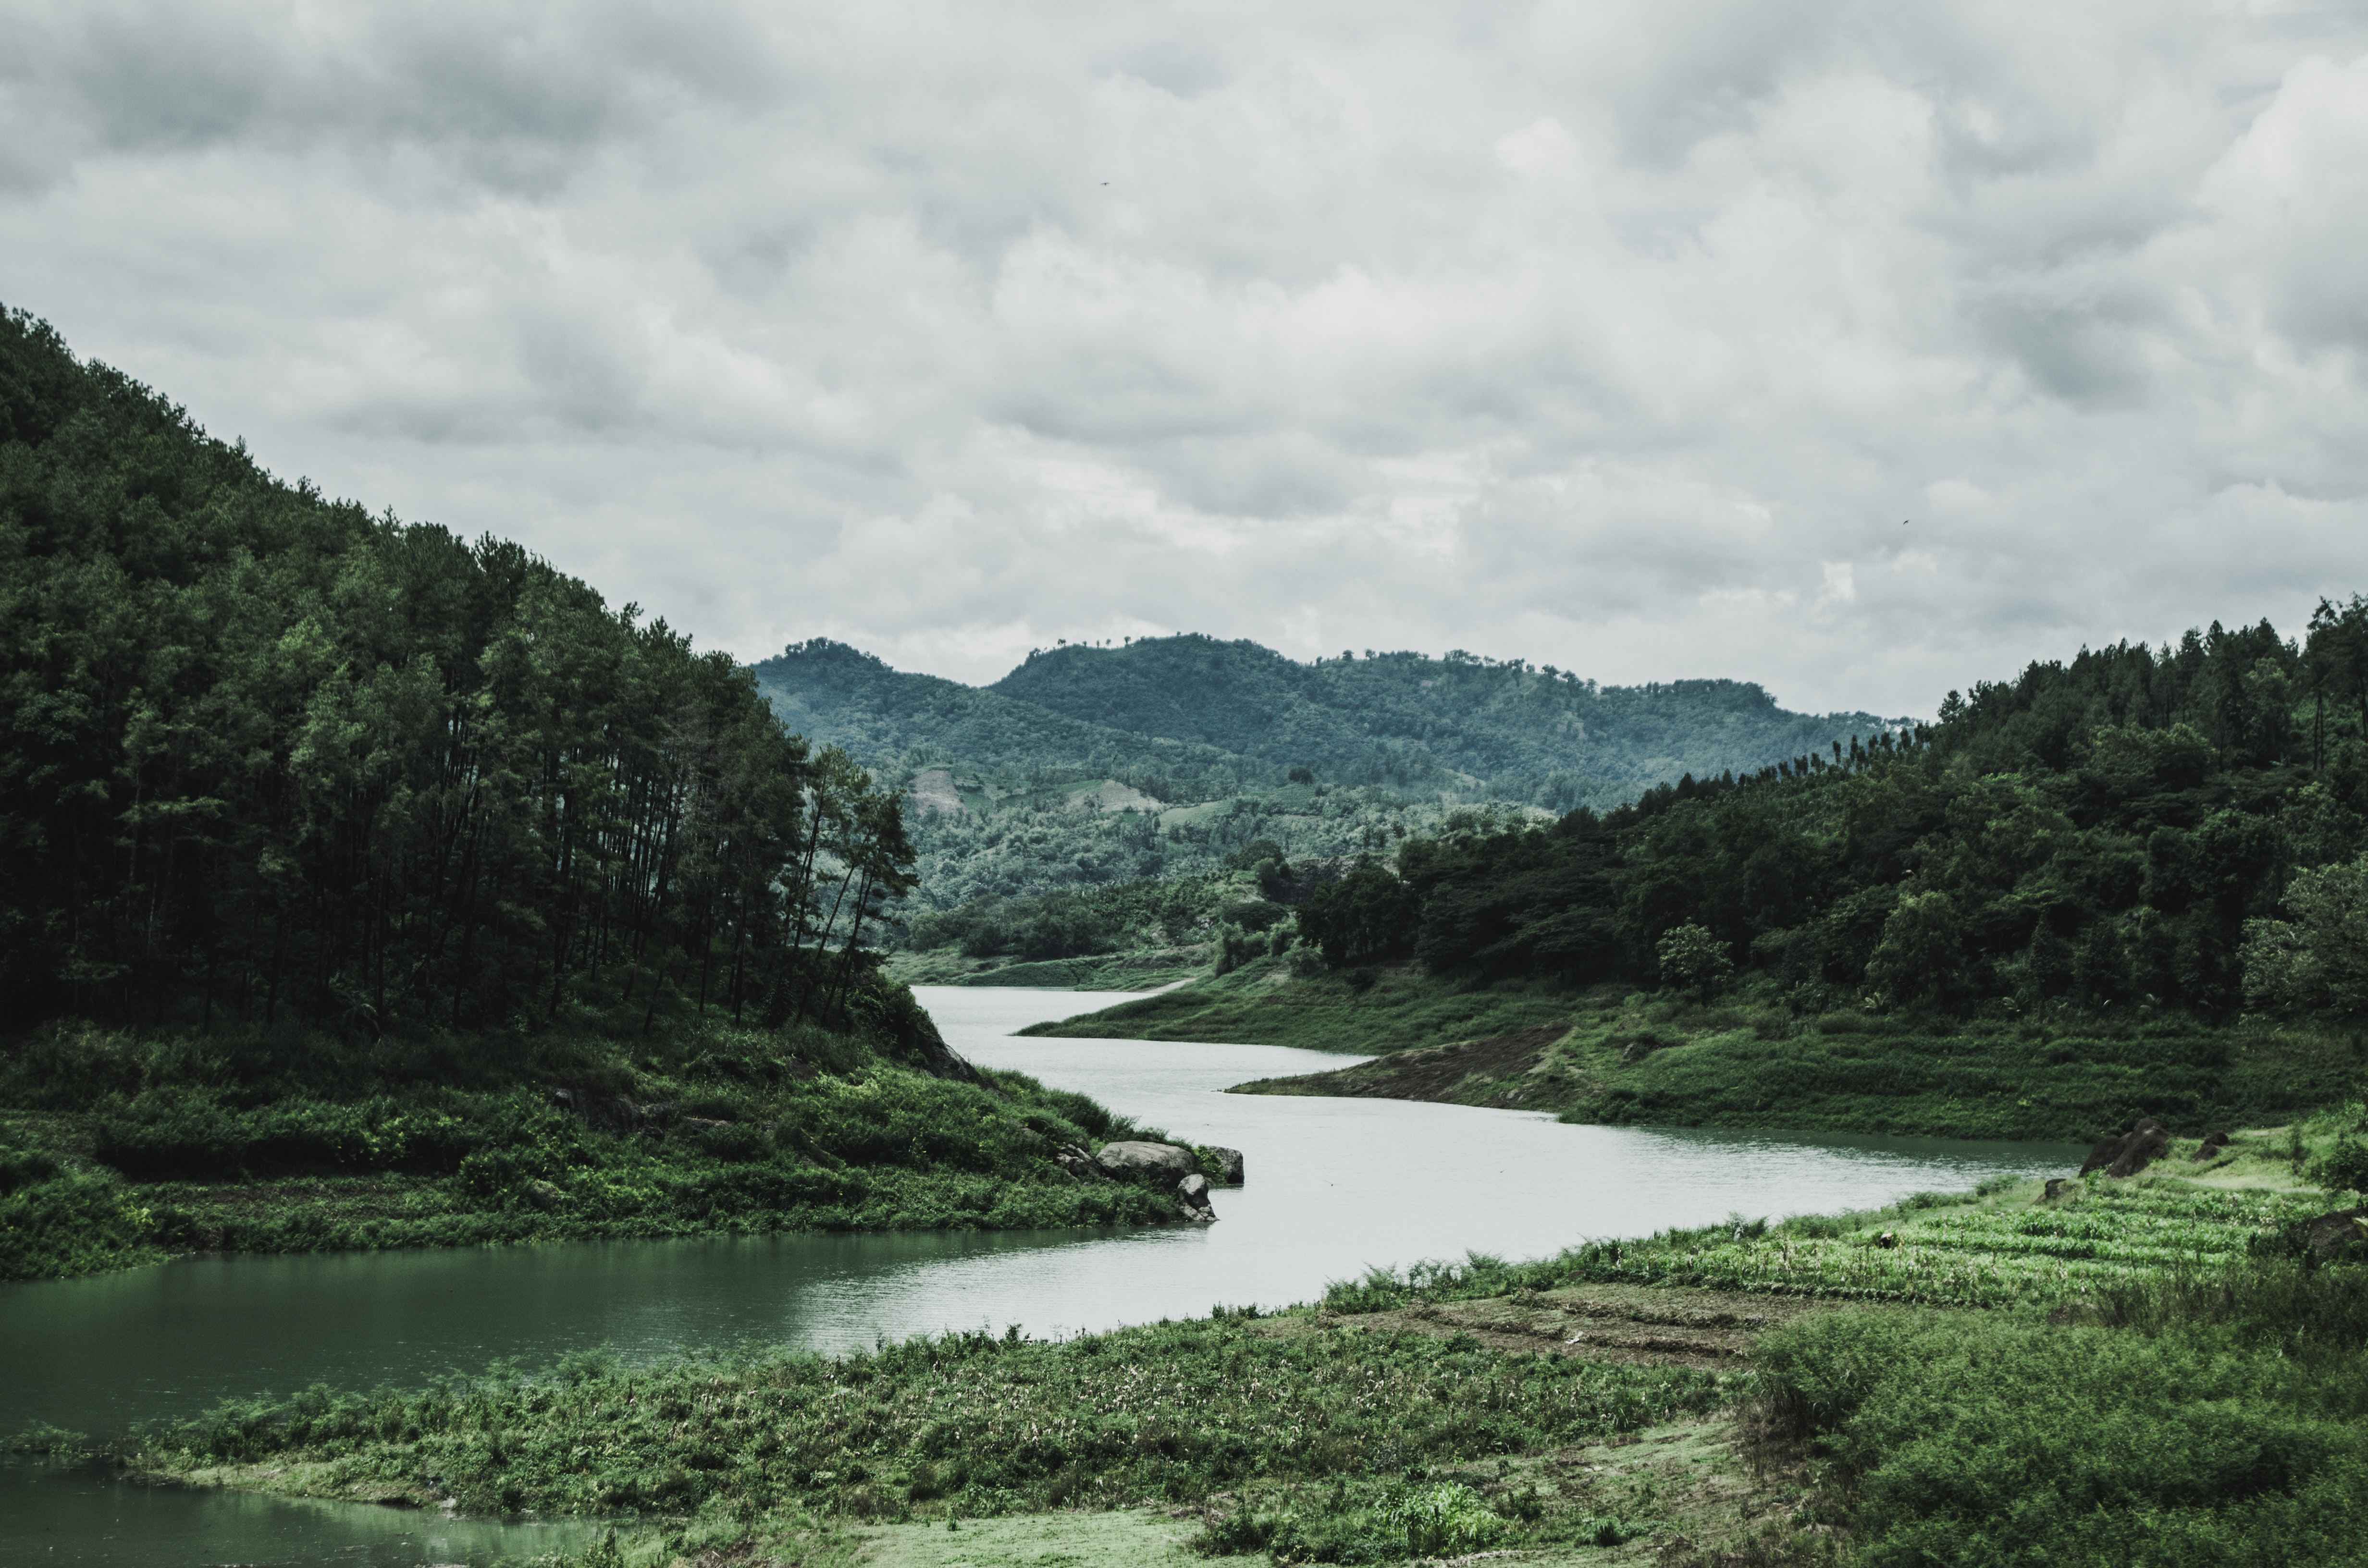
\includegraphics[width=\textwidth]{images/pexels-rido-alwarno-1034887.jpg}
            \caption{A river.}
            \label{fig:01_river}
        \end{subfigure}
        \hfill
        \begin{subfigure}[b]{0.45\textwidth}
            \centering
            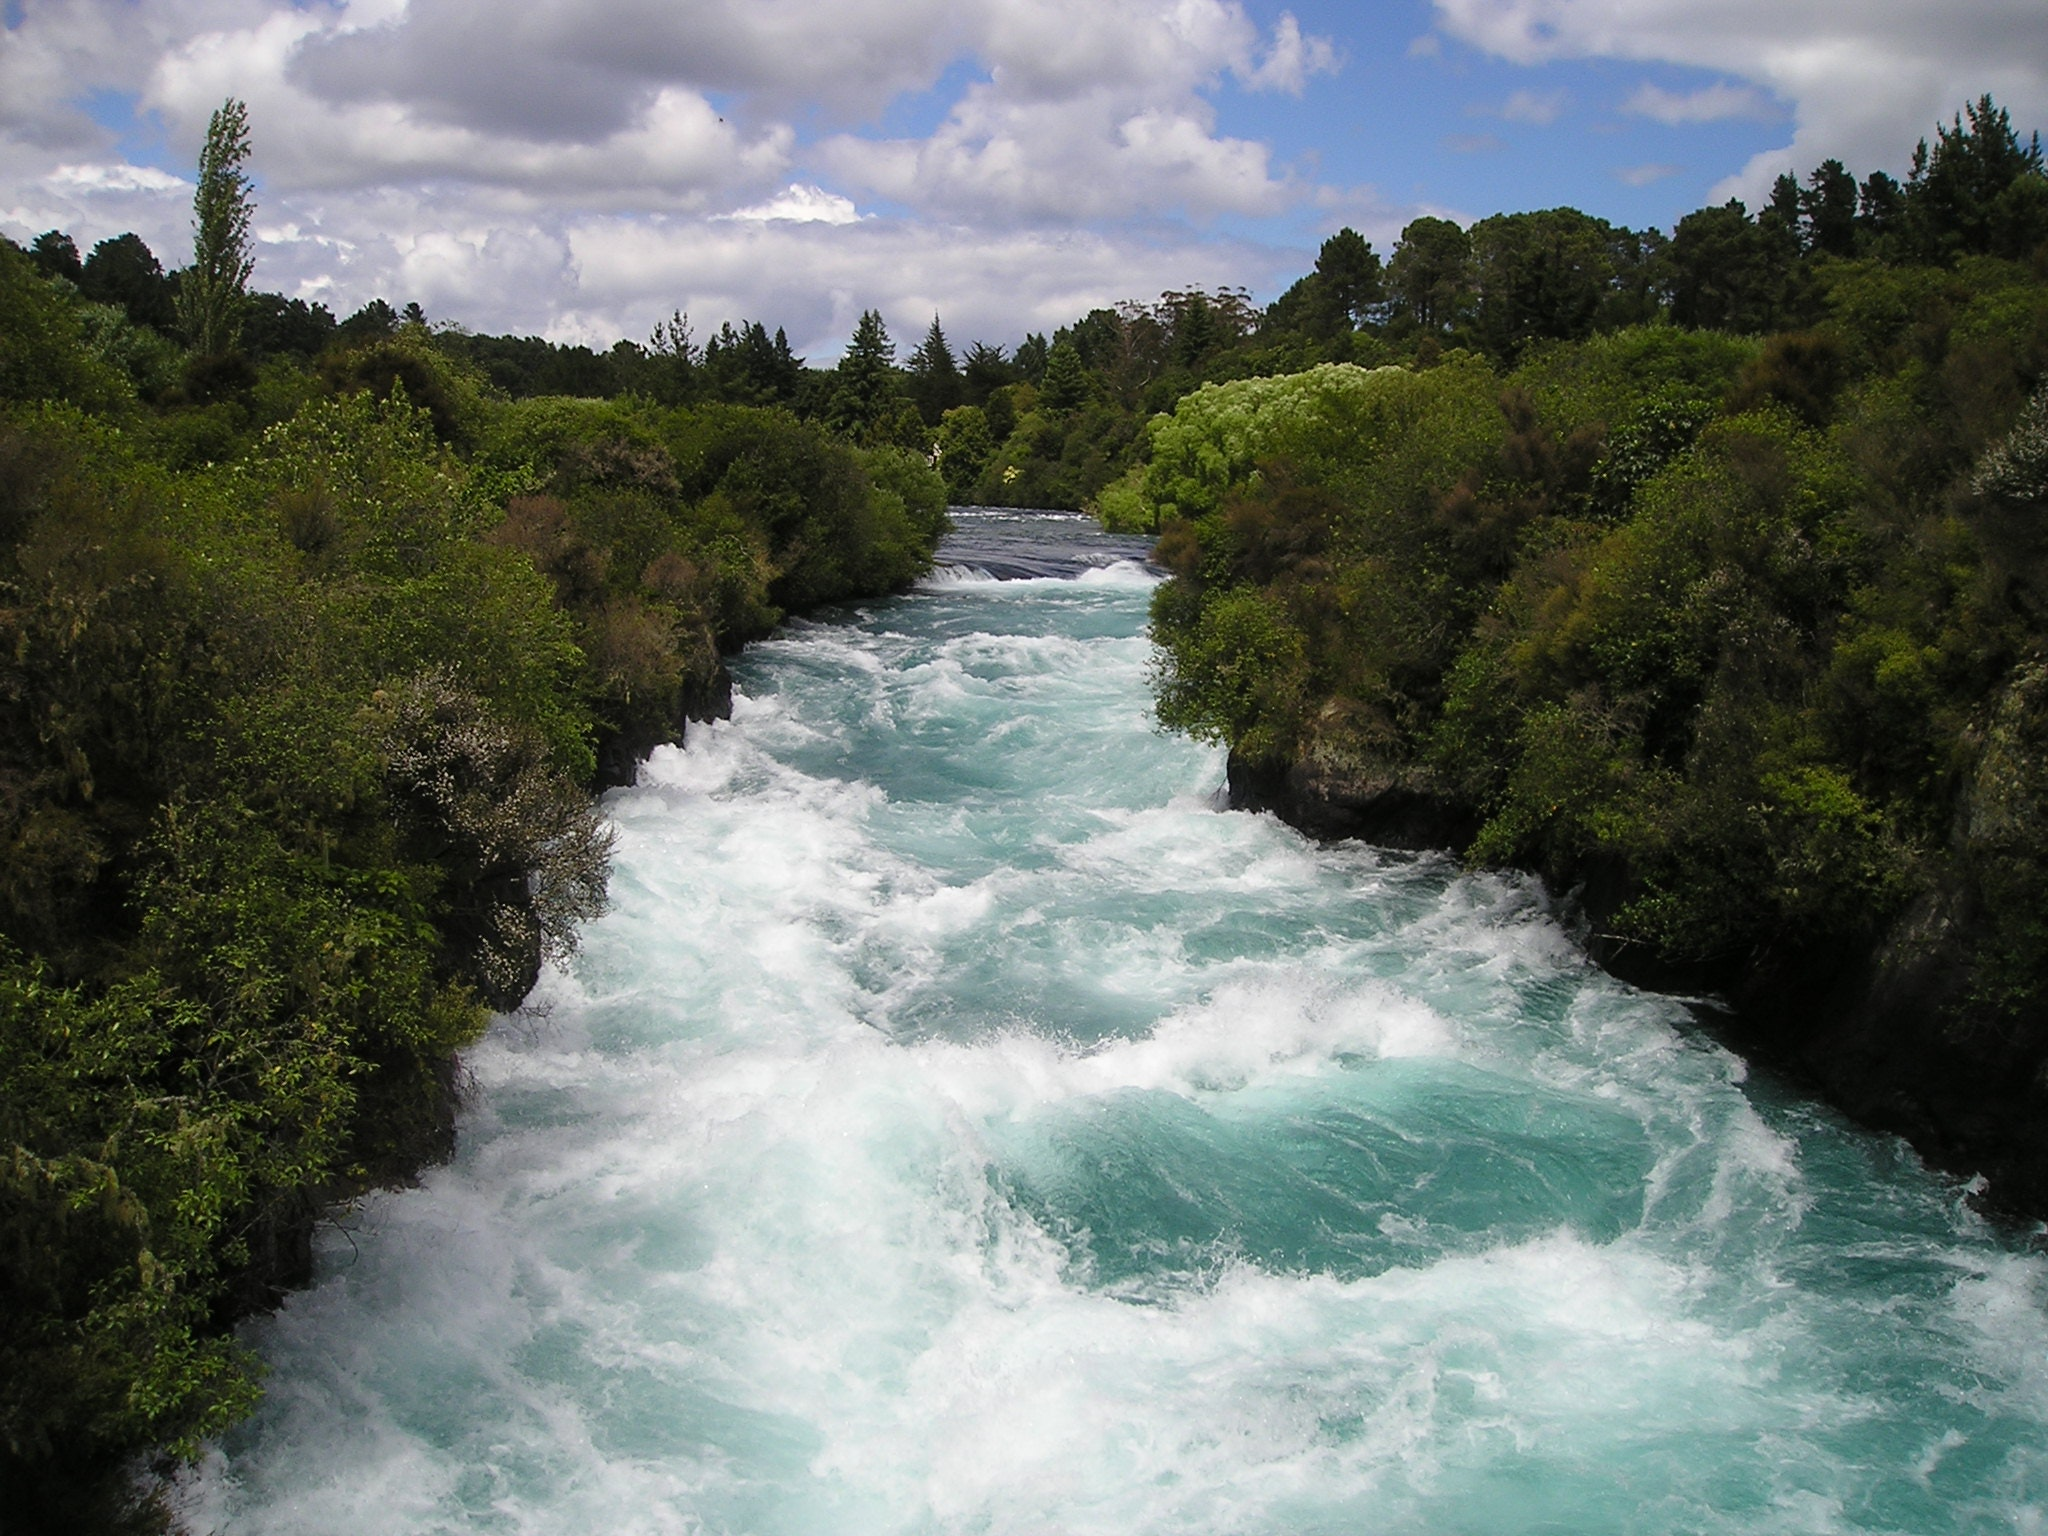
\includegraphics[width=\textwidth]{images/pexels-pixabay-2438.jpg}
            \caption{An angry river.}
            \label{fig:01_angry_river}
        \end{subfigure}
        \caption{Natural wave phenomena.}
        \label{fig:rivers}
    \end{figure}
\end{frame}